\documentclass{article}% [Determines font size] { }Determines type of document (article/beamer/book/etc.)

\usepackage{graphicx}% Required package to compile figures.
\usepackage{blindtext}

\begin{document}% Required to produce a compiled LaTeX document. 

\blindtext

\begin{figure}% This creates a separate environment for the figure, independent of the rest of the document. [ ] are placing options of where in the page/environment should the figure be displayed, and when to overwrite other established rules. 
    \caption{Complete figure format}% Creates a title for the figure, with an automatically generating ordered number placement of the figure. To place the title below the figure, then place the \caption command after \includegraphics.
    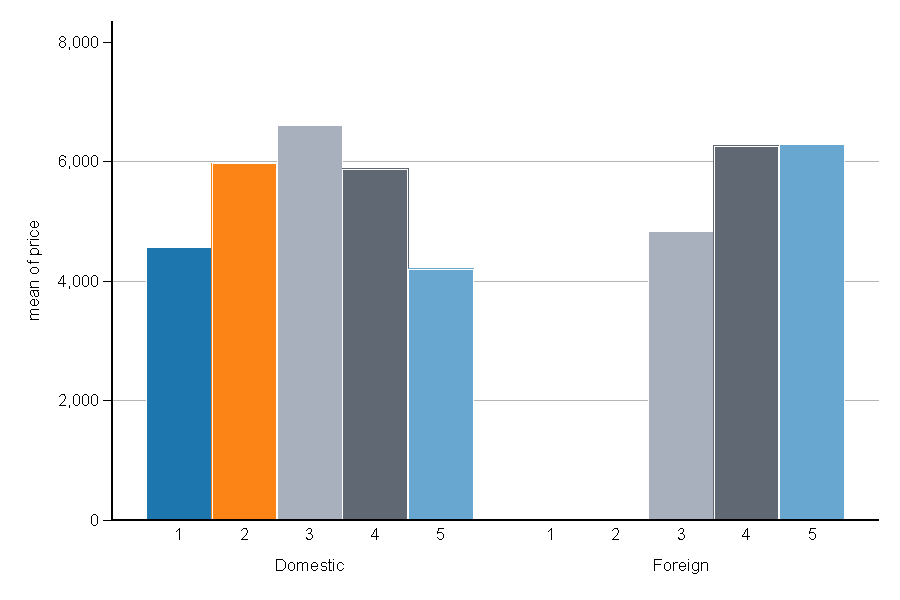
\includegraphics[width=\textwidth]{figure1.pdf}% [ ] used to customize the size of the figure displayed in document. 
    \label{fig:placements_none}%Use a ":" to create a category of labels on the left side, and the right side is the label of this specific figure.
\end{figure}

\blindtext

\newpage

\blindtext

\begin{figure}[h]% 
    \caption{Complete figure format}% 
    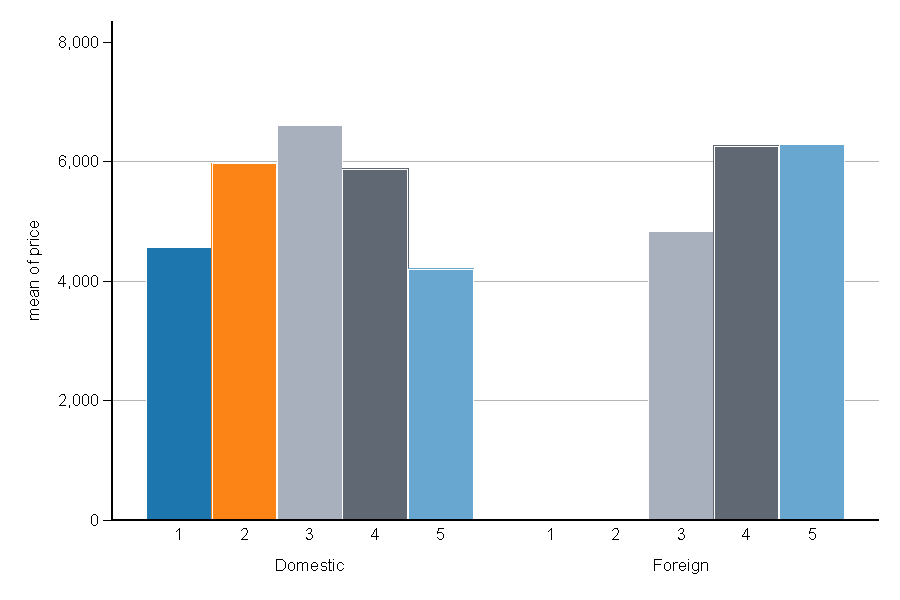
\includegraphics[width=1\textwidth]{figure1.pdf}% 
    \label{fig:placements_h}%
\end{figure}

\blindtext

\newpage

\blindtext

\begin{figure}[t]% 
    \caption{Complete figure format}% 
    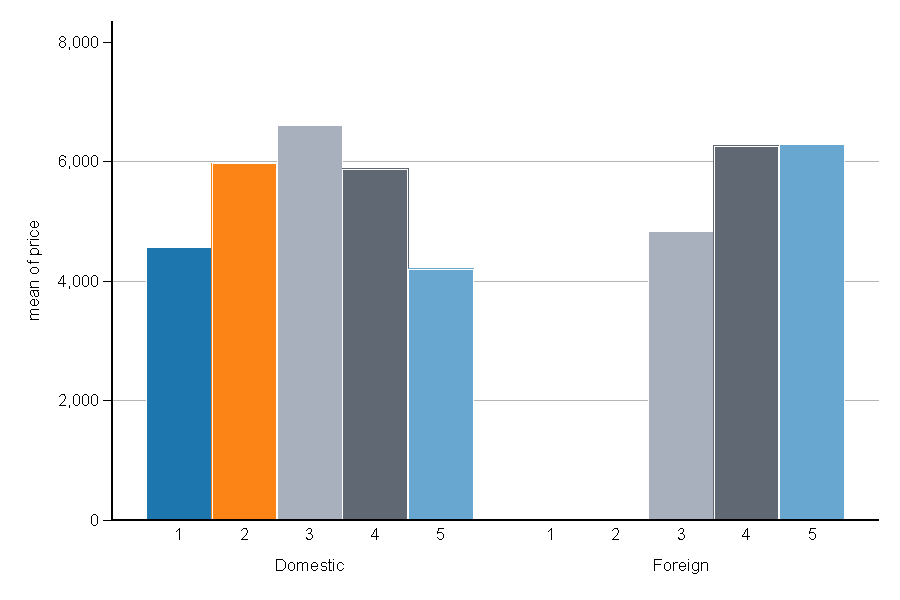
\includegraphics[width=1\textwidth]{figure1.pdf}% 
    \label{fig:placements_t}%
\end{figure}

\blindtext


\blindtext

\begin{figure}[!b]% 
    \caption{Complete figure format}% 
    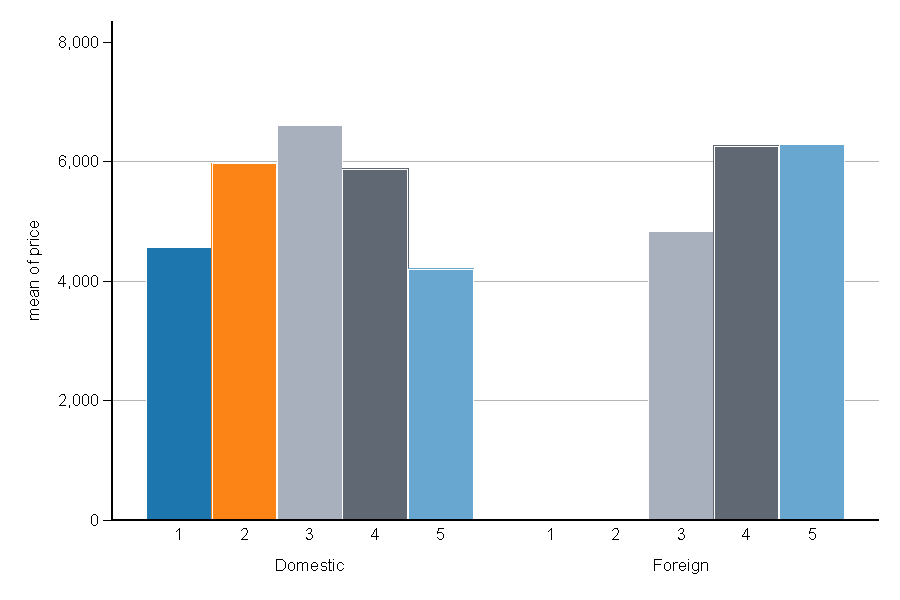
\includegraphics[width=1\textwidth]{figure1.pdf}% 
    \label{fig:placements_b}%
\end{figure}

\blindtext

\newpage

\blindtext

\begin{figure}[p]% 
    \caption{Complete figure format}% 
    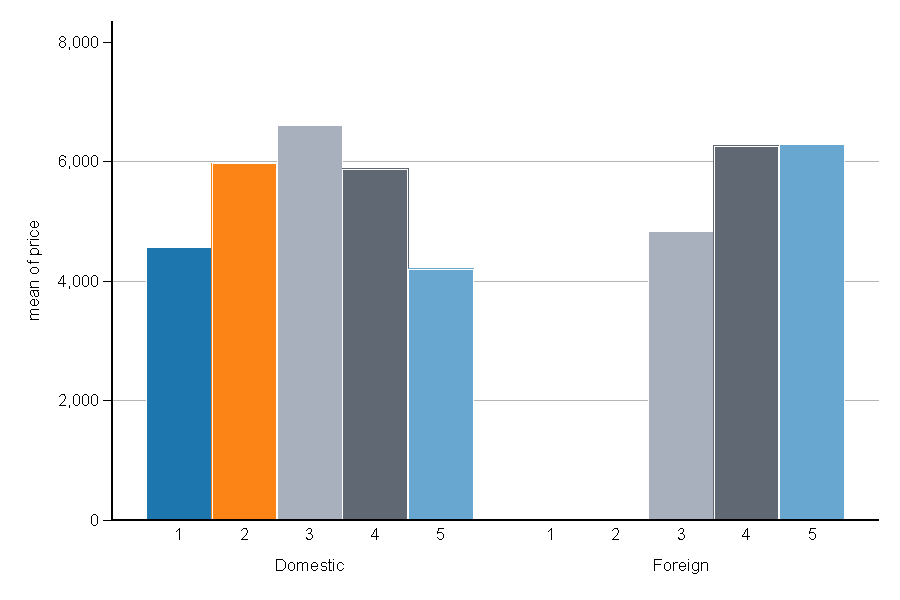
\includegraphics[width=1\textwidth]{figure1.pdf}% 
    \label{fig:placements_p}%
\end{figure}

\blindtext


\end{document}